\section{Angular Momentum}

\subsection{Orbital angular momentum}

\subsubsection{Classical orbital angular momentum}

\begin{wrapfigure}{r}{0.5\textwidth}
  \centering
  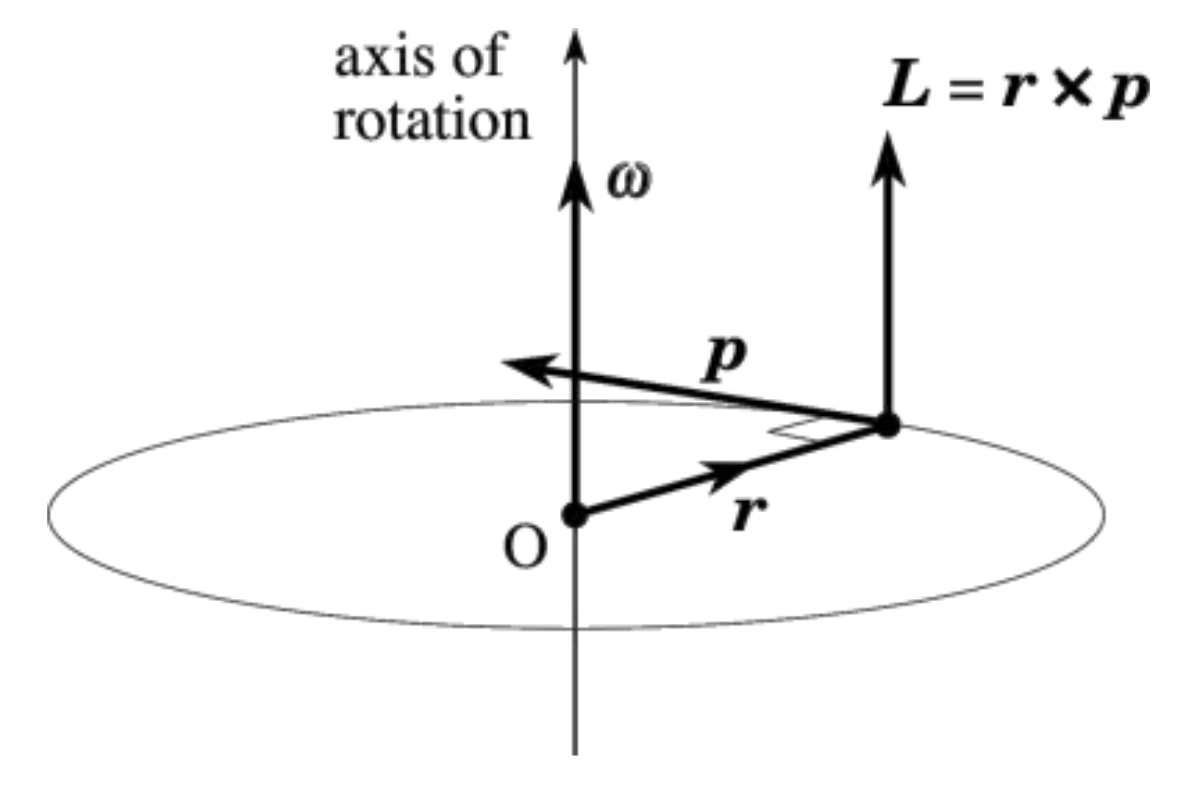
\includegraphics[width=0.5\textwidth]{images/classical_angular_momentum.png}
  \caption{Classical orbital angular momentum}
  \label{fig:classical_angular_momentum}
\end{wrapfigure}

In classical mechanics, the angular momentum of a particle relative to some axis is defined as:

\begin{equation}
    \vec{L} = \vec{r} \times \vec{p}
\end{equation}

where $\vec{r}$ is the position vector of the particle with respect to a point on the axis of rotation and $\vec{p}$ is its momentum. 

The total angular momentum of a system of particles is the sum of angular momenta of the individual particles:
\begin{equation}
    \vec{L}_\text{total} = \sum_i \vec{r}_i \times \vec{p}_i
\end{equation}

The total angular momentum varies in time according to the net external torque, which we can obtain by differentiating the total angular momentum with respect to time:
\begin{equation}
    \vec{\tau}_\text{total} = \sum_i \vec{\tau}_{\text{ext},i} = \frac{d\vec{L}_\text{total}}{dt}
\end{equation}

It follows that the total angular momentum of a system is conserved if the resultant external torque acting on the system is zero.

\subsubsection{Orbital angular momentum in quantum mechanics}

As discussed in \textbf{Section \ref{observables_and_operators}}, to obtain the quantum mechanical operator for orbital angular momentum from its classical definition, we can apply quantization to the classical expression provided in the previous section:
\begin{equation}
    \vec{L} = \vec{R} \times \vec{P} = -i\hbar \vec{R}\times \vec{\nabla}
\end{equation}

For a system of (spin-less) particles, the total angular momentum is defined as:
\begin{equation}
    \vec{L}_\text{total} = \sum_i \vec{R}_i \times \vec{P}_i
\end{equation}

The different cartesian components of the angular momentum operator are:
\begin{equation}
    \begin{split}
        L_x &= YP_z - ZP_y = -i\hbar \left(Y\frac{\partial}{\partial z} - Z\frac{\partial}{\partial y}\right) \\
        L_y &= ZP_x - XP_z = -i\hbar \left(Z\frac{\partial}{\partial x} - X\frac{\partial}{\partial z}\right) \\
        L_z &= XP_y - YP_x = -i\hbar \left(X\frac{\partial}{\partial y} - Y\frac{\partial}{\partial x}\right)
    \end{split}
\end{equation}
We can also define the square of the angular momentum operator:
\begin{equation}
    L^2 = L_x^2 + L_y^2 + L_z^2
\end{equation}
As expected from operators corresponding to observables, all angular momentum operators are Hermitian.

\subsubsection{Commutation relations}

The commutation relations for the orbital angular momentum operators are:
\begin{equation}
    \begin{split}
        [L_x, L_y] &= L_xL_y - L_yL_x = i\hbar L_z \\
        [L_y, L_z] &= L_yL_z - L_zL_y = i\hbar L_x \\
        [L_z, L_x] &= L_zL_x - L_xL_z = i\hbar L_y
    \end{split}
\end{equation}

\subsubsection{General formalism of angular momentum}

We have just defined the orbital angular momentum. However there exists a more general formalism of angular momentum, which is the \textit{total} angular momentum. Its corresponding operator is $\vec{J}$, defined by its three components that satisfy:
\begin{equation} \label{eq:commutation_relations_angular_momentum}
    \begin{split}
        [J_x, J_y] &= i\hbar J_z \\
        [J_y, J_z] &= i\hbar J_x \\
        [J_z, J_x] &= i\hbar J_y
    \end{split}\qquad \vec{J}\,^2 = J_x^2 + J_y^2 + J_z^2\qquad [\vec{J}\,^2, J_k] = 0\quad (k = x, y, z)
\end{equation}

Thanks to these commutation relations, we know that we cannot measure the three components of the total angular momentum simultaneously. However, we \textit{can} simultaneously measure the total angular momentum squared $J^2$ and one of its components. There is possibility to find simultaneous eigenstates of $J^2$ and any component of $J$. However, we can only choose one component of $J$ to be measured simultaneously with $J^2$. By convention, we choose $J_z$, so that we work with a basis of eigenvectors that is common to $J^2$ and $J_z$ in all our calculations\footnote{Note that this is just a convention. There is \textit{nothing} special about the $z$ direction compared to $x$ and $y$.}.

\textit{Eigenstates of the total angular momentum operators}

Let us now look for the joint eigenstates of $J^2$ and $J_z$ and their corresponding eigenvalues. Denoting the joint eigenstates by $\ket{\alpha, \beta}$, and the corresponding eigenvalues of $J^2$ and $J_z$ by $\hbar^2\alpha$ and $\hbar \beta$, respectively, we have:
\begin{equation} \label{eq:angular_momentum_eigenstates}
    \begin{split}
        J^2\ket{\alpha, \beta} &= \hbar^2\alpha\ket{\alpha, \beta} \\
        J_z\ket{\alpha, \beta} &= \hbar\beta\ket{\alpha, \beta}
    \end{split}
\end{equation}
The factor $\hbar$ is introduced so that $\alpha$ and $\beta$ are dimensionless. We also assume that the eigenstates are orthonormal.

Now we need to introduce \textit{raising} and \textit{lowering} operators $J_+$ and $J_-$, respectively, which are defined as:
\begin{equation}
    J_\pm = J_x \pm iJ_y
\end{equation}
This leads to:
\begin{equation}
    J_x = \frac12(J_+ + J_-)\qquad J_y = \frac{1}{2i}(J_+ - J_-)
\end{equation}
hence:
\begin{equation}
    J_x^2 = \frac14(J_+^2+J_+J_-+J_-J_++J_-^2)\qquad J_y^2 = -\frac{1}{4}(J_+^2-J_+J_--J_-J_++J_-^2)
\end{equation}
Using the commutation relations from \textbf{Equation \ref{eq:commutation_relations_angular_momentum}}, we can easily obtain:
\begin{equation} \label{eq:commutation_relations_angular_momentum_2}
    [\vec{J}\,^2, J_\pm] = 0\qquad [J_+, J_-] = 2\hbar J_z \qquad [J_z, J_\pm] = \pm\hbar J_\pm
\end{equation}
And also:
\begin{equation} \label{j_p_and_j_m_products}
    \begin{split}
        J_+J_- = J_x^2 + J_y^2 + \hbar J_z = \vec{J}\,^2 - J_z^2 + \hbar J_z\\
        J_-J_+ = J_x^2 + J_y^2 - \hbar J_z = \vec{J}\,^2 - J_z^2 - \hbar J_z
    \end{split} 
\end{equation}
These relations lead to:
\begin{equation}
    \vec{J}\,^2 = J_\pm J_\mp + J_z^2 \mp \hbar J_z = \frac12(J_+ J_- + J_- J_+) + J_z^2
\end{equation}

Since $J_\pm$ do not commute with $J_z$, the kets $\ket{\alpha, \beta}$ are not eigenstates of $J_\pm$. Using the expressions in \textbf{Equation \ref{eq:commutation_relations_angular_momentum_2}}, we can obtain:
\begin{equation} \label{eq:jz_jpm_eigenstates}
    \begin{split}
        J_z(J_\pm\ket{\alpha, \beta}) &= (J_\pm J_z \pm \hbar J_\pm)\ket{\alpha, \beta} = J_\pm J_z \ket{\alpha, \beta} \pm \hbar J_\pm \ket{\alpha, \beta} = \\
        &= \hbar \beta J_\pm \ket{\alpha, \beta} \pm \hbar J_\pm \ket{\alpha, \beta} = \hbar(\beta \pm 1)(J_\pm\ket{\alpha, \beta})
    \end{split}
\end{equation} 
hence the ket $J_\pm\ket{\alpha, \beta}$ is an eigenstate of $J_z$ with eigenvalue $\hbar(\beta \pm 1)$. Since $\vec{J}\,^2$ commutes with $J_z$, $J_\pm\ket{\alpha, \beta}$ is also an eigenstate of $\vec{J}\,^2$. Using \textbf{Equation \ref{eq:commutation_relations_angular_momentum_2}} again, which tells us that $\vec{J}\,^2$ commutes with $J_\pm$, we can determine the eigenvalue, which is $\hbar^2\alpha$:
\begin{equation} \label{eq:j2_jpm_eigenstates}
    \vec{J}\,^2(J_\pm\ket{\alpha, \beta}) = J_\pm \vec{J}\,^2\ket{\alpha, \beta} = J_\pm \hbar^2\alpha \ket{\alpha, \beta} = \hbar^2\alpha(J_\pm \ket{\alpha, \beta})
\end{equation}

If we rewrite \textbf{Equation \ref{eq:jz_jpm_eigenstates}} and \textbf{Equation \ref{eq:j2_jpm_eigenstates}} in terms of $\ket{\alpha',\beta'} = J_\pm \ket{\alpha,\beta}$:
\begin{equation}
    \begin{split}
        J_z\ket{\alpha', \beta'} &= \hbar(\beta \pm 1)\ket{\alpha', \beta'} \\
        \vec{J}\,^2\ket{\alpha', \beta'} &= \hbar^2\alpha\ket{\alpha', \beta'}
    \end{split}
\end{equation}

and if we compare with \textbf{Equation \ref{eq:angular_momentum_eigenstates}}, we can infer that $\alpha' = \alpha$ and $\beta' = \beta \pm 1$. In other words, the ket $J_\pm\ket{\alpha,\beta}$ is proportional to $\ket{\alpha, \beta\pm 1}$ (any eigenket multiplied by a constant is also an eigenket, although it may not be normalised), and we can write:
\begin{equation} \label{eq:j_p_and_j_m_eigenstates}
    J_\pm\ket{\alpha, \beta} = C_{\alpha\beta}^\pm\ket{\alpha, \beta\pm 1}
\end{equation}

So, when the operators $J_\pm$ act on a ket $\ket{\alpha, \beta}$, they do not change the first quantum number $\alpha$, but they increase (or decrease) the second quantum number $\beta$ by one unit. Hence the names \textit{raising} and \textit{lowering} operators.

Note that, for a given eigenvalue $\alpha$ of $\vec{J}\,^2$, there exists an upper limit for the \textit{absolute value}\footnote{That is to say, $\beta$ is bounded from above \textit{and} below.} of the quantum number $\beta$. This is due to the fact that the operator $\vec{J}\,^2 - J_z^2$ is positive definite, as the matrix elements of $\vec{J}\,^2 - J_z^2 = J_x^2 + J_y^2 \geq 0$ are non-negative, so we can write:
\begin{equation}
    \braket{\alpha, \beta| \vec{J}\,^2 - J_z^2 | \alpha, \beta} = \hbar^2(\alpha - \beta^2) \geq 0\quad \Longrightarrow\quad \alpha \geq\beta^2
\end{equation} 

Since $\beta$ has an upper limit, $\beta_\text{max}$, there must exist a state $\ket{\alpha, \beta_\text{max}}$ which cannot be raised further:
\begin{equation}
    J_+\ket{\alpha, \beta_\text{max}} = 0
\end{equation}

Using this, along with \textbf{Equation \ref{j_p_and_j_m_products}}, we can obtain:
\begin{equation}
    J_-J_+\ket{\alpha,\beta_\text{max}} = (\vec{J}\,^2 - J_z^2 - \hbar J_z)\ket{\alpha,\beta_\text{max}} = \hbar^2(\alpha-\beta_\text{max}^2 - \beta_\text{max})\ket{\alpha,\beta_\text{max}} = 0
\end{equation}
hence:
\begin{equation}
    \alpha = \beta_\text{max}(\beta_\text{max} + 1)
\end{equation}

Since $\beta$ has a lower limit, $\beta_\text{min}$, there must exist a state $\ket{\alpha, \beta_\text{min}}$ which cannot be lowered further, which we reach after $n$ successive applications of $J_-$ on $\ket{\alpha, \beta_\text{max}}$:
\begin{equation} \label{eq:alpha_beta_max}
    J_-\ket{\alpha, \beta_\text{min}} = 0
\end{equation}

Using this, along with \textbf{Equation \ref{j_p_and_j_m_products}}, we can obtain:
\begin{equation}
    J_+J_-\ket{\alpha,\beta_\text{min}} = (\vec{J}\,^2 - J_z^2 + \hbar J_z)\ket{\alpha,\beta_\text{min}} = \hbar^2(\alpha-\beta_\text{min}^2 + \beta_\text{min})\ket{\alpha,\beta_\text{min}} = 0
\end{equation}
hence:
\begin{equation} \label{eq:alpha_beta_min}
    \alpha = \beta_\text{min}(\beta_\text{min} - 1)
\end{equation}

Comparing \textbf{Equation \ref{eq:alpha_beta_max}} and \textbf{Equation \ref{eq:alpha_beta_min}}, we can infer that:
\begin{equation}
    \beta_\text{max} = -\beta_\text{min}
\end{equation}

Since $\beta_\text{min}$ was reached after $n$ successive applications of $J_-$ on $\ket{\alpha, \beta_\text{max}}$, it follows that:
\begin{equation}
    \beta_\text{max} = \beta_\text{min} + n, \qquad n\in \N
\end{equation}

Combining the last two equations, we obtain:
\begin{equation}
    \beta_\text{min} = -\frac{n}{2}\qquad \beta_\text{max} = \frac{n}{2}
\end{equation}

Which means that $\beta_\text{max}$ is either an integer or a half-odd-integer. We can now introduce the notation:
\begin{equation}
    j = \beta_\text{max} = \frac{n}{2}\qquad m = \beta
\end{equation}
hence, we can express $\alpha$ as:
\begin{equation}
    \alpha = j(j+1)
\end{equation}m = -j, -j+1, \dots, j-1, j
And we can infer that the values of $m$ lie between $-j$ and $j$:
\begin{equation}
    -j \leq m \leq j
\end{equation}

We can now summarize the results we have obtained so far:
\begin{definition}
    The eigenvalues of $\vec{J}\,^2$ and $J_z$ corresponding to the joint eigenvectors $\ket{j,m}$ are given, respectively, by $\hbar^2j(j+1)$ and $\hbar m$:
    \begin{equation}
        \vec{J}\,^2\ket{j,m} = \hbar^2j(j+1)\ket{j,m}\qquad J_z\ket{j,m} = \hbar m\ket{j,m}
    \end{equation}
    where $j = 0,\, 1/2,\, 1,\, 3/2,\, ...$ and $m = -j, -(j-1), \dots, j-1, j$. We see that the spectra of the angular momentum operators $\vec{J}\,^2$ and $J_z$ are discrete. Since the eigenstates corresponding to different angular momenta are orthogonal, and since the angular momentum spectra are discrete, the orthonormality condition is:
    \begin{equation}
        \braket{j',m'|j,m} = \delta_{j',j}\delta_{m',m}
    \end{equation}
\end{definition}

Let us now determine the normalization constant $C_{\alpha\beta}^\pm$ in \textbf{Equation \ref{eq:j_p_and_j_m_eigenstates}}, which we can rewrite in terms of $j$ and $m$ as:
\begin{equation}
    J_\pm\ket{j,m} = C_{jm}^\pm\ket{j,m\pm 1}
\end{equation}
Since $\ket{j,m+1}$ is normalized:
\begin{equation}
    (J_+\ket{j,m})^\dagger (J_+\ket{j,m}) = |C_{jm}^+|^2\braket{j, m+1|j, m+1} = |C_{jm}^+|^2
\end{equation}

Since $J_+ = J_x + iJ_y$ and the operators $J_x$ and $J_y$ are Hermitian, we have:
\begin{equation}
    J_+^\dagger = (J_x+iJ_y)^\dagger = J_x^\dagger -iJ_y^\dagger = J_x - iJ_y = J_-
\end{equation}
So we can also write:
\begin{equation}
    \braket{j,m|J_-J_+|j,m} = \braket{j,m|J_+^\dagger J_+|j,m} = (J_+\ket{j,m})^\dagger (J_+\ket{j,m}) = |C_{jm}^+|^2
\end{equation}

But since $J_-J_+ = \vec{J}\,^2 - J_z^2 - \hbar J_z$ and $\ket{j,m}$ is orthonormal, we can also write:

\begin{equation}
    \begin{split}
        |C_{jm}^+|^2 &= \braket{j,m|J_-J_+|j,m} = \braket{j,m|\vec{J}\,^2 - J_z^2 - \hbar J_z|j,m} = \\
        &= \braket{j,m|\vec{J}\,^2|j,m} - \braket{j,m|J_z^2|j,m} - \hbar\braket{j,m|J_z|j,m} = \\
        &= \braket{j,m|\hbar^2j(j+1)|j,m} - \braket{j,m|\hbar^2m^2|j,m} - \hbar\braket{j,m|\hbar m|j,m} = \\
        &= \hbar^2j(j+1)\braket{j,m|j,m} - \hbar^2m^2\braket{j,m|j,m} - \hbar^2m\braket{j,m|j,m} = \\
        &= \hbar^2j(j+1) - \hbar^2m^2 - \hbar^2m \\
        &= \hbar^2(j(j+1)-m(m+1))
    \end{split}
\end{equation}

So we conclude that\footnote{Note that here we would actually have to add a phase factor $e^{i\theta}$ so that $C_{jm}^+ = \hbar \sqrt{j(j+1)-m(m+1)}e^{i\theta}$. This is beacuse $C_{jm}^+$ is, in general terms, a complex number. As we have the freedom of choice, we take $C_{jm}^+$ to be real and positive. The same argument applies to $C_{jm}^-$.}:
\begin{equation}
    C_{jm}^+ = \hbar \sqrt{j(j+1)-m(m+1)}
\end{equation}

Similarly, we can obtain:
\begin{equation}
    C_{jm}^- = \hbar \sqrt{j(j+1)-m(m-1)}
\end{equation}

So, we now have the raising and lowering operators completely defined:
\begin{definition}
    The raising and lowering operators $J_+$ and $J_-$ are given by:
    \begin{equation}
        J_\pm = J_x \pm iJ_y
    \end{equation}
    Their action on a ket $\ket{j,m}$ raises or lowers the second quantum number $m$ by one unit, respectively:
    \begin{equation}
        J_\pm\ket{j,m} = \hbar \sqrt{j(j+1)-m(m\pm1)}\ket{j,m\pm 1}
    \end{equation}
\end{definition}